\documentclass[twoside]{book}

% Packages required by doxygen
\usepackage{fixltx2e}
\usepackage{calc}
\usepackage{doxygen}
\usepackage[export]{adjustbox} % also loads graphicx
\usepackage{graphicx}
\usepackage[utf8]{inputenc}
\usepackage{makeidx}
\usepackage{multicol}
\usepackage{multirow}
\PassOptionsToPackage{warn}{textcomp}
\usepackage{textcomp}
\usepackage[nointegrals]{wasysym}
\usepackage[table]{xcolor}

% Font selection
\usepackage[T1]{fontenc}
\usepackage[scaled=.90]{helvet}
\usepackage{courier}
\usepackage{amssymb}
\usepackage{sectsty}
\renewcommand{\familydefault}{\sfdefault}
\allsectionsfont{%
  \fontseries{bc}\selectfont%
  \color{darkgray}%
}
\renewcommand{\DoxyLabelFont}{%
  \fontseries{bc}\selectfont%
  \color{darkgray}%
}
\newcommand{\+}{\discretionary{\mbox{\scriptsize$\hookleftarrow$}}{}{}}

% Page & text layout
\usepackage{geometry}
\geometry{%
  a4paper,%
  top=2.5cm,%
  bottom=2.5cm,%
  left=2.5cm,%
  right=2.5cm%
}
\tolerance=750
\hfuzz=15pt
\hbadness=750
\setlength{\emergencystretch}{15pt}
\setlength{\parindent}{0cm}
\setlength{\parskip}{3ex plus 2ex minus 2ex}
\makeatletter
\renewcommand{\paragraph}{%
  \@startsection{paragraph}{4}{0ex}{-1.0ex}{1.0ex}{%
    \normalfont\normalsize\bfseries\SS@parafont%
  }%
}
\renewcommand{\subparagraph}{%
  \@startsection{subparagraph}{5}{0ex}{-1.0ex}{1.0ex}{%
    \normalfont\normalsize\bfseries\SS@subparafont%
  }%
}
\makeatother

% Headers & footers
\usepackage{fancyhdr}
\pagestyle{fancyplain}
\fancyhead[LE]{\fancyplain{}{\bfseries\thepage}}
\fancyhead[CE]{\fancyplain{}{}}
\fancyhead[RE]{\fancyplain{}{\bfseries\leftmark}}
\fancyhead[LO]{\fancyplain{}{\bfseries\rightmark}}
\fancyhead[CO]{\fancyplain{}{}}
\fancyhead[RO]{\fancyplain{}{\bfseries\thepage}}
\fancyfoot[LE]{\fancyplain{}{}}
\fancyfoot[CE]{\fancyplain{}{}}
\fancyfoot[RE]{\fancyplain{}{\bfseries\scriptsize Generated by Doxygen }}
\fancyfoot[LO]{\fancyplain{}{\bfseries\scriptsize Generated by Doxygen }}
\fancyfoot[CO]{\fancyplain{}{}}
\fancyfoot[RO]{\fancyplain{}{}}
\renewcommand{\footrulewidth}{0.4pt}
\renewcommand{\chaptermark}[1]{%
  \markboth{#1}{}%
}
\renewcommand{\sectionmark}[1]{%
  \markright{\thesection\ #1}%
}

% Indices & bibliography
\usepackage{natbib}
\usepackage[titles]{tocloft}
\setcounter{tocdepth}{3}
\setcounter{secnumdepth}{5}
\makeindex

% Hyperlinks (required, but should be loaded last)
\usepackage{ifpdf}
\ifpdf
  \usepackage[pdftex,pagebackref=true]{hyperref}
\else
  \usepackage[ps2pdf,pagebackref=true]{hyperref}
\fi
\hypersetup{%
  colorlinks=true,%
  linkcolor=blue,%
  citecolor=blue,%
  unicode%
}

% Custom commands
\newcommand{\clearemptydoublepage}{%
  \newpage{\pagestyle{empty}\cleardoublepage}%
}

\usepackage{caption}
\captionsetup{labelsep=space,justification=centering,font={bf},singlelinecheck=off,skip=4pt,position=top}

%===== C O N T E N T S =====

\begin{document}

% Titlepage & ToC
\hypersetup{pageanchor=false,
             bookmarksnumbered=true,
             pdfencoding=unicode
            }
\pagenumbering{alph}
\begin{titlepage}
\vspace*{7cm}
\begin{center}%
{\Large Sigil Tools }\\
\vspace*{1cm}
{\large Generated by Doxygen 1.8.12}\\
\end{center}
\end{titlepage}
\clearemptydoublepage
\pagenumbering{roman}
\tableofcontents
\clearemptydoublepage
\pagenumbering{arabic}
\hypersetup{pageanchor=true}

%--- Begin generated contents ---
\chapter{Hierarchical Index}
\section{Class Hierarchy}
This inheritance list is sorted roughly, but not completely, alphabetically\+:\begin{DoxyCompactList}
\item \contentsline{section}{Color}{\pageref{struct_color}}{}
\item \contentsline{section}{P\+Vector}{\pageref{struct_p_vector}}{}
\item \contentsline{section}{Shape}{\pageref{class_shape}}{}
\begin{DoxyCompactList}
\item \contentsline{section}{Circle\+Shape}{\pageref{class_circle_shape}}{}
\item \contentsline{section}{Polygon}{\pageref{class_polygon}}{}
\item \contentsline{section}{Rectangle\+Shape}{\pageref{class_rectangle_shape}}{}
\item \contentsline{section}{Triangle\+Shape}{\pageref{class_triangle_shape}}{}
\end{DoxyCompactList}
\end{DoxyCompactList}

\chapter{Class Index}
\section{Class List}
Here are the classes, structs, unions and interfaces with brief descriptions\+:\begin{DoxyCompactList}
\item\contentsline{section}{\hyperlink{class_circle_shape}{Circle\+Shape} }{\pageref{class_circle_shape}}{}
\item\contentsline{section}{\hyperlink{struct_color}{Color} }{\pageref{struct_color}}{}
\item\contentsline{section}{\hyperlink{class_polygon}{Polygon} }{\pageref{class_polygon}}{}
\item\contentsline{section}{\hyperlink{struct_p_vector}{P\+Vector} }{\pageref{struct_p_vector}}{}
\item\contentsline{section}{\hyperlink{class_rectangle_shape}{Rectangle\+Shape} }{\pageref{class_rectangle_shape}}{}
\item\contentsline{section}{\hyperlink{class_shape}{Shape} }{\pageref{class_shape}}{}
\item\contentsline{section}{\hyperlink{class_triangle_shape}{Triangle\+Shape} }{\pageref{class_triangle_shape}}{}
\end{DoxyCompactList}

\chapter{File Index}
\section{File List}
Here is a list of all files with brief descriptions\+:\begin{DoxyCompactList}
\item\contentsline{section}{\hyperlink{_tools_8cpp}{Tools.\+cpp} }{\pageref{_tools_8cpp}}{}
\item\contentsline{section}{\hyperlink{_tools_8hpp}{Tools.\+hpp} }{\pageref{_tools_8hpp}}{}
\end{DoxyCompactList}

\chapter{Class Documentation}
\hypertarget{class_circle_shape}{}\section{Circle\+Shape Class Reference}
\label{class_circle_shape}\index{Circle\+Shape@{Circle\+Shape}}


{\ttfamily \#include $<$Tools.\+hpp$>$}

Inheritance diagram for Circle\+Shape\+:\begin{figure}[H]
\begin{center}
\leavevmode
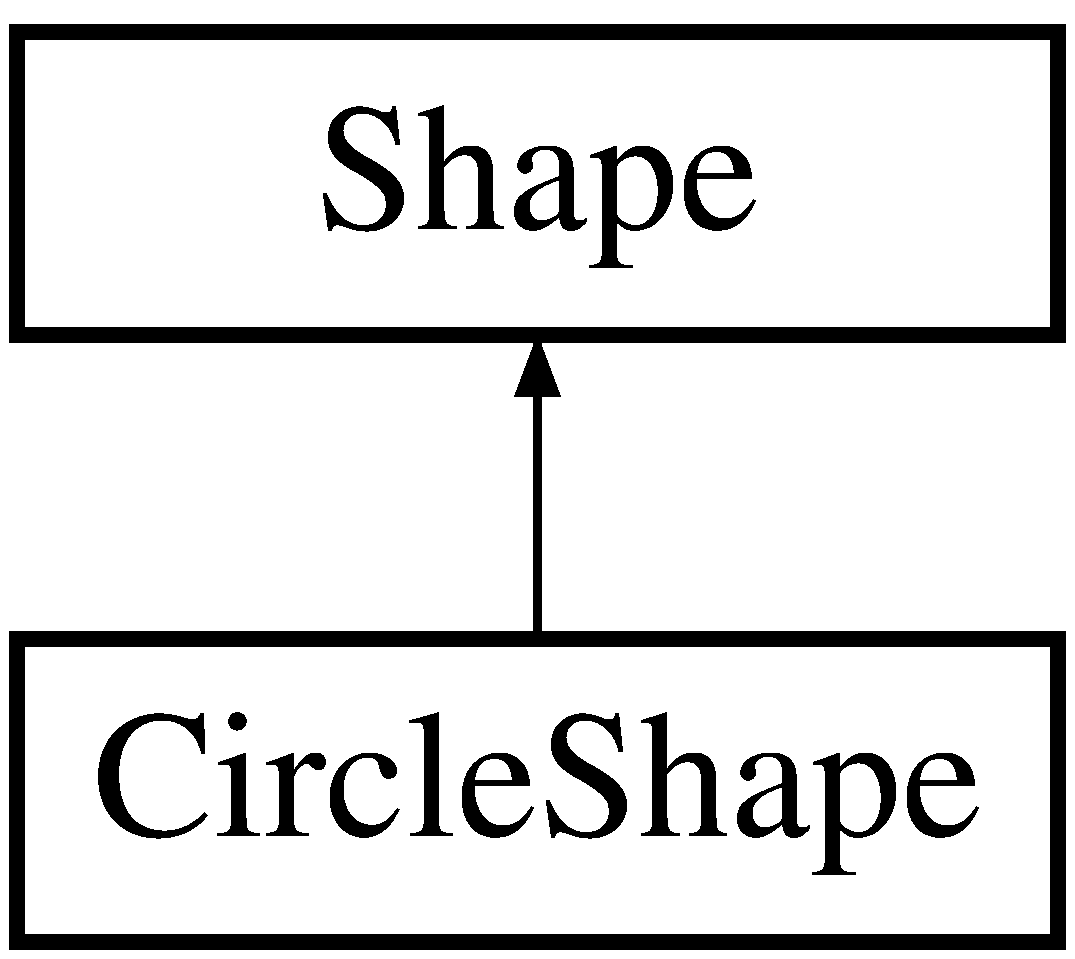
\includegraphics[height=2.000000cm]{class_circle_shape}
\end{center}
\end{figure}
\subsection*{Public Member Functions}
\begin{DoxyCompactItemize}
\item 
\hyperlink{class_circle_shape_a4e5614b889576afbd5c744ca39129a73}{Circle\+Shape} (float, float, float)
\item 
void \hyperlink{class_circle_shape_a4bdbdab71c47dd560ba58b4d21659be1}{draw\+Fill} ()
\item 
void \hyperlink{class_circle_shape_a42fe963aa4872668748f0ba882f49878}{draw\+Outline} ()
\item 
void \hyperlink{class_circle_shape_af317d58be28370ba183df07734fde939}{set\+Radius} (float)
\item 
float \hyperlink{class_circle_shape_a931eb9fffe6985d45717bf8175960503}{get\+Radius} ()
\end{DoxyCompactItemize}
\subsection*{Additional Inherited Members}


\subsection{Constructor \& Destructor Documentation}
\hypertarget{class_circle_shape_a4e5614b889576afbd5c744ca39129a73}{}\label{class_circle_shape_a4e5614b889576afbd5c744ca39129a73} 
\index{Circle\+Shape@{Circle\+Shape}!Circle\+Shape@{Circle\+Shape}}
\index{Circle\+Shape@{Circle\+Shape}!Circle\+Shape@{Circle\+Shape}}
\subsubsection{\texorpdfstring{Circle\+Shape()}{CircleShape()}}
{\footnotesize\ttfamily Circle\+Shape\+::\+Circle\+Shape (\begin{DoxyParamCaption}\item[{float}]{x = {\ttfamily 0},  }\item[{float}]{y = {\ttfamily 0},  }\item[{float}]{r = {\ttfamily 0} }\end{DoxyParamCaption})}



\subsection{Member Function Documentation}
\hypertarget{class_circle_shape_a4bdbdab71c47dd560ba58b4d21659be1}{}\label{class_circle_shape_a4bdbdab71c47dd560ba58b4d21659be1} 
\index{Circle\+Shape@{Circle\+Shape}!draw\+Fill@{draw\+Fill}}
\index{draw\+Fill@{draw\+Fill}!Circle\+Shape@{Circle\+Shape}}
\subsubsection{\texorpdfstring{draw\+Fill()}{drawFill()}}
{\footnotesize\ttfamily void Circle\+Shape\+::draw\+Fill (\begin{DoxyParamCaption}{ }\end{DoxyParamCaption})}

\hypertarget{class_circle_shape_a42fe963aa4872668748f0ba882f49878}{}\label{class_circle_shape_a42fe963aa4872668748f0ba882f49878} 
\index{Circle\+Shape@{Circle\+Shape}!draw\+Outline@{draw\+Outline}}
\index{draw\+Outline@{draw\+Outline}!Circle\+Shape@{Circle\+Shape}}
\subsubsection{\texorpdfstring{draw\+Outline()}{drawOutline()}}
{\footnotesize\ttfamily void Circle\+Shape\+::draw\+Outline (\begin{DoxyParamCaption}{ }\end{DoxyParamCaption})}

\hypertarget{class_circle_shape_a931eb9fffe6985d45717bf8175960503}{}\label{class_circle_shape_a931eb9fffe6985d45717bf8175960503} 
\index{Circle\+Shape@{Circle\+Shape}!get\+Radius@{get\+Radius}}
\index{get\+Radius@{get\+Radius}!Circle\+Shape@{Circle\+Shape}}
\subsubsection{\texorpdfstring{get\+Radius()}{getRadius()}}
{\footnotesize\ttfamily float Circle\+Shape\+::get\+Radius (\begin{DoxyParamCaption}{ }\end{DoxyParamCaption})}

\hypertarget{class_circle_shape_af317d58be28370ba183df07734fde939}{}\label{class_circle_shape_af317d58be28370ba183df07734fde939} 
\index{Circle\+Shape@{Circle\+Shape}!set\+Radius@{set\+Radius}}
\index{set\+Radius@{set\+Radius}!Circle\+Shape@{Circle\+Shape}}
\subsubsection{\texorpdfstring{set\+Radius()}{setRadius()}}
{\footnotesize\ttfamily void Circle\+Shape\+::set\+Radius (\begin{DoxyParamCaption}\item[{float}]{r }\end{DoxyParamCaption})}



The documentation for this class was generated from the following files\+:\begin{DoxyCompactItemize}
\item 
\hyperlink{_tools_8hpp}{Tools.\+hpp}\item 
\hyperlink{_tools_8cpp}{Tools.\+cpp}\end{DoxyCompactItemize}

\hypertarget{struct_color}{}\section{Color Struct Reference}
\label{struct_color}\index{Color@{Color}}


{\ttfamily \#include $<$Tools.\+hpp$>$}

\subsection*{Public Member Functions}
\begin{DoxyCompactItemize}
\item 
\hyperlink{struct_color_a90c33a7c6af6542e917c8fb136c59bd3}{Color} (float, float, float, float)
\item 
void \hyperlink{struct_color_ab277df545876e66a8094fd5d3dbbcaf2}{set\+Fore\+Color} ()
\end{DoxyCompactItemize}
\subsection*{Public Attributes}
\begin{DoxyCompactItemize}
\item 
float \hyperlink{struct_color_a3958a556b47d2de3dd45c75aac833c20}{r}
\item 
float \hyperlink{struct_color_a5defbb21620e480e556181772d665f34}{g}
\item 
float \hyperlink{struct_color_a33e482be18d6ea31d2b403bee13683b7}{b}
\item 
float \hyperlink{struct_color_a98047aee65fc3d825f88a76da728fd27}{a}
\end{DoxyCompactItemize}


\subsection{Constructor \& Destructor Documentation}
\hypertarget{struct_color_a90c33a7c6af6542e917c8fb136c59bd3}{}\label{struct_color_a90c33a7c6af6542e917c8fb136c59bd3} 
\index{Color@{Color}!Color@{Color}}
\index{Color@{Color}!Color@{Color}}
\subsubsection{\texorpdfstring{Color()}{Color()}}
{\footnotesize\ttfamily Color\+::\+Color (\begin{DoxyParamCaption}\item[{float}]{red = {\ttfamily 1},  }\item[{float}]{green = {\ttfamily 1},  }\item[{float}]{blue = {\ttfamily 1},  }\item[{float}]{alpha = {\ttfamily 1} }\end{DoxyParamCaption})}



\subsection{Member Function Documentation}
\hypertarget{struct_color_ab277df545876e66a8094fd5d3dbbcaf2}{}\label{struct_color_ab277df545876e66a8094fd5d3dbbcaf2} 
\index{Color@{Color}!set\+Fore\+Color@{set\+Fore\+Color}}
\index{set\+Fore\+Color@{set\+Fore\+Color}!Color@{Color}}
\subsubsection{\texorpdfstring{set\+Fore\+Color()}{setForeColor()}}
{\footnotesize\ttfamily void Color\+::set\+Fore\+Color (\begin{DoxyParamCaption}{ }\end{DoxyParamCaption})}



\subsection{Member Data Documentation}
\hypertarget{struct_color_a98047aee65fc3d825f88a76da728fd27}{}\label{struct_color_a98047aee65fc3d825f88a76da728fd27} 
\index{Color@{Color}!a@{a}}
\index{a@{a}!Color@{Color}}
\subsubsection{\texorpdfstring{a}{a}}
{\footnotesize\ttfamily float Color\+::a}

\hypertarget{struct_color_a33e482be18d6ea31d2b403bee13683b7}{}\label{struct_color_a33e482be18d6ea31d2b403bee13683b7} 
\index{Color@{Color}!b@{b}}
\index{b@{b}!Color@{Color}}
\subsubsection{\texorpdfstring{b}{b}}
{\footnotesize\ttfamily float Color\+::b}

\hypertarget{struct_color_a5defbb21620e480e556181772d665f34}{}\label{struct_color_a5defbb21620e480e556181772d665f34} 
\index{Color@{Color}!g@{g}}
\index{g@{g}!Color@{Color}}
\subsubsection{\texorpdfstring{g}{g}}
{\footnotesize\ttfamily float Color\+::g}

\hypertarget{struct_color_a3958a556b47d2de3dd45c75aac833c20}{}\label{struct_color_a3958a556b47d2de3dd45c75aac833c20} 
\index{Color@{Color}!r@{r}}
\index{r@{r}!Color@{Color}}
\subsubsection{\texorpdfstring{r}{r}}
{\footnotesize\ttfamily float Color\+::r}



The documentation for this struct was generated from the following files\+:\begin{DoxyCompactItemize}
\item 
\hyperlink{_tools_8hpp}{Tools.\+hpp}\item 
\hyperlink{_tools_8cpp}{Tools.\+cpp}\end{DoxyCompactItemize}

\hypertarget{class_polygon}{}\section{Polygon Class Reference}
\label{class_polygon}\index{Polygon@{Polygon}}
Inheritance diagram for Polygon\+:\begin{figure}[H]
\begin{center}
\leavevmode
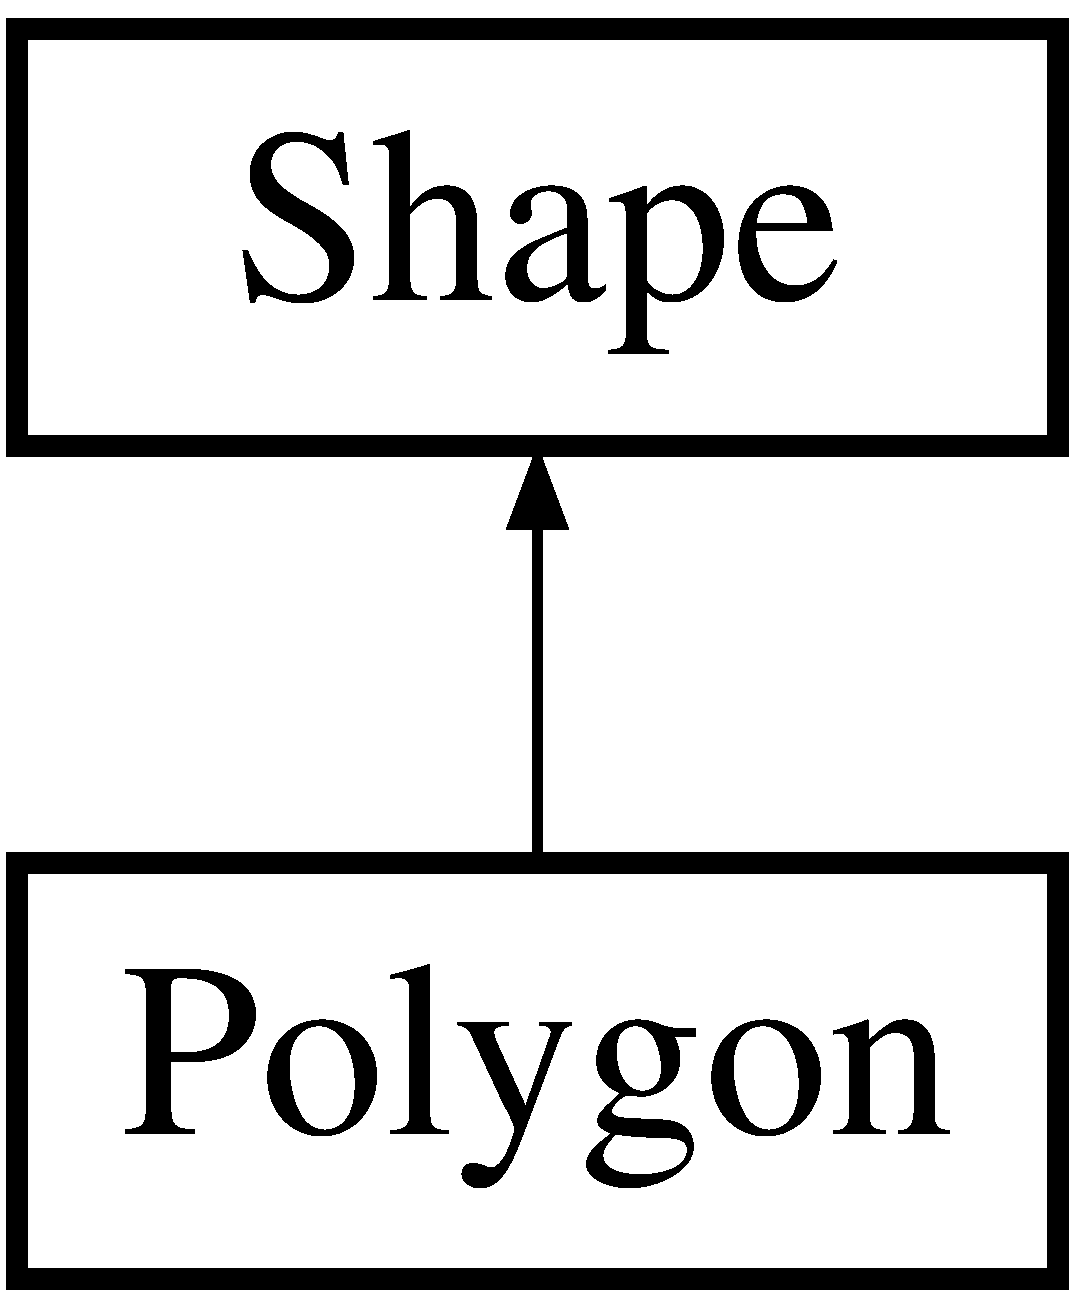
\includegraphics[height=2.000000cm]{class_polygon}
\end{center}
\end{figure}
\subsection*{Public Member Functions}
\begin{DoxyCompactItemize}
\item 
\hypertarget{class_polygon_a8ba4cc1def2c799bb4e75df1aa6fbb72}{}\label{class_polygon_a8ba4cc1def2c799bb4e75df1aa6fbb72} 
{\bfseries Polygon} (float, float, int)
\item 
\hypertarget{class_polygon_a3ae4366cd72f2414f133fab680983ea9}{}\label{class_polygon_a3ae4366cd72f2414f133fab680983ea9} 
void {\bfseries draw\+Outline} ()
\item 
\hypertarget{class_polygon_a55580fc352e83e29d3bc2679e5d8bdbf}{}\label{class_polygon_a55580fc352e83e29d3bc2679e5d8bdbf} 
void {\bfseries set\+Point} (int, \hyperlink{struct_p_vector}{P\+Vector})
\item 
\hypertarget{class_polygon_a5423331a39f62cf1382b9465bfa170aa}{}\label{class_polygon_a5423331a39f62cf1382b9465bfa170aa} 
\hyperlink{struct_p_vector}{P\+Vector} {\bfseries get\+Point} (int)
\item 
\hypertarget{class_polygon_ad269b9c3f239834cd24235c73dd31bab}{}\label{class_polygon_ad269b9c3f239834cd24235c73dd31bab} 
int {\bfseries get\+Point\+Count} ()
\end{DoxyCompactItemize}
\subsection*{Additional Inherited Members}


The documentation for this class was generated from the following files\+:\begin{DoxyCompactItemize}
\item 
Tools.\+hpp\item 
Tools.\+cpp\end{DoxyCompactItemize}

\hypertarget{struct_p_vector}{}\section{P\+Vector Struct Reference}
\label{struct_p_vector}\index{P\+Vector@{P\+Vector}}


{\ttfamily \#include $<$Tools.\+hpp$>$}

\subsection*{Public Member Functions}
\begin{DoxyCompactItemize}
\item 
\hyperlink{struct_p_vector_aaed7f72779101199eb499892e000f7e8}{P\+Vector} (float, float)
\end{DoxyCompactItemize}
\subsection*{Public Attributes}
\begin{DoxyCompactItemize}
\item 
float \hyperlink{struct_p_vector_ae8b1d40fd11089e7949cb333cf949d13}{x}
\item 
float \hyperlink{struct_p_vector_a63d91c43b923e9e63f1fb1e0598b5962}{y}
\end{DoxyCompactItemize}


\subsection{Constructor \& Destructor Documentation}
\hypertarget{struct_p_vector_aaed7f72779101199eb499892e000f7e8}{}\label{struct_p_vector_aaed7f72779101199eb499892e000f7e8} 
\index{P\+Vector@{P\+Vector}!P\+Vector@{P\+Vector}}
\index{P\+Vector@{P\+Vector}!P\+Vector@{P\+Vector}}
\subsubsection{\texorpdfstring{P\+Vector()}{PVector()}}
{\footnotesize\ttfamily P\+Vector\+::\+P\+Vector (\begin{DoxyParamCaption}\item[{float}]{x = {\ttfamily 0},  }\item[{float}]{y = {\ttfamily 0} }\end{DoxyParamCaption})}



\subsection{Member Data Documentation}
\hypertarget{struct_p_vector_ae8b1d40fd11089e7949cb333cf949d13}{}\label{struct_p_vector_ae8b1d40fd11089e7949cb333cf949d13} 
\index{P\+Vector@{P\+Vector}!x@{x}}
\index{x@{x}!P\+Vector@{P\+Vector}}
\subsubsection{\texorpdfstring{x}{x}}
{\footnotesize\ttfamily float P\+Vector\+::x}

\hypertarget{struct_p_vector_a63d91c43b923e9e63f1fb1e0598b5962}{}\label{struct_p_vector_a63d91c43b923e9e63f1fb1e0598b5962} 
\index{P\+Vector@{P\+Vector}!y@{y}}
\index{y@{y}!P\+Vector@{P\+Vector}}
\subsubsection{\texorpdfstring{y}{y}}
{\footnotesize\ttfamily float P\+Vector\+::y}



The documentation for this struct was generated from the following files\+:\begin{DoxyCompactItemize}
\item 
\hyperlink{_tools_8hpp}{Tools.\+hpp}\item 
\hyperlink{_tools_8cpp}{Tools.\+cpp}\end{DoxyCompactItemize}

\hypertarget{class_rectangle_shape}{}\section{Rectangle\+Shape Class Reference}
\label{class_rectangle_shape}\index{Rectangle\+Shape@{Rectangle\+Shape}}
Inheritance diagram for Rectangle\+Shape\+:\begin{figure}[H]
\begin{center}
\leavevmode
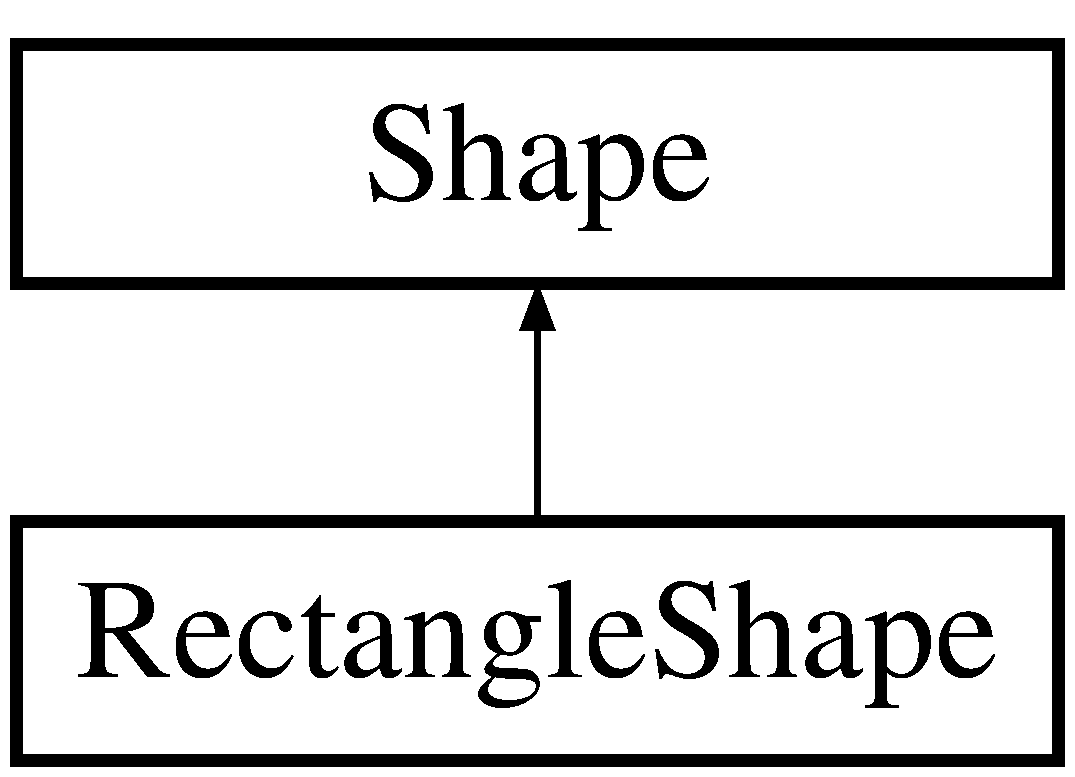
\includegraphics[height=2.000000cm]{class_rectangle_shape}
\end{center}
\end{figure}
\subsection*{Public Member Functions}
\begin{DoxyCompactItemize}
\item 
\hypertarget{class_rectangle_shape_aaca6ad79b0f0f6a2cdd3b07cb7d132ed}{}\label{class_rectangle_shape_aaca6ad79b0f0f6a2cdd3b07cb7d132ed} 
{\bfseries Rectangle\+Shape} (float, float, float, float)
\item 
\hypertarget{class_rectangle_shape_a5981b643c3f26733159e92910eaa25ee}{}\label{class_rectangle_shape_a5981b643c3f26733159e92910eaa25ee} 
void {\bfseries draw\+Fill} ()
\item 
\hypertarget{class_rectangle_shape_af4c688f1ad48c2ba76970d93d19f5b4b}{}\label{class_rectangle_shape_af4c688f1ad48c2ba76970d93d19f5b4b} 
void {\bfseries draw\+Outline} ()
\item 
\hypertarget{class_rectangle_shape_a8736f7ba16291db873ad9d31570bba06}{}\label{class_rectangle_shape_a8736f7ba16291db873ad9d31570bba06} 
void {\bfseries set\+Size} (\hyperlink{struct_p_vector}{P\+Vector})
\item 
\hypertarget{class_rectangle_shape_a4788f9784e80e4bfbfa913207d98c558}{}\label{class_rectangle_shape_a4788f9784e80e4bfbfa913207d98c558} 
\hyperlink{struct_p_vector}{P\+Vector} {\bfseries get\+Size} ()
\end{DoxyCompactItemize}
\subsection*{Additional Inherited Members}


The documentation for this class was generated from the following files\+:\begin{DoxyCompactItemize}
\item 
Tools.\+hpp\item 
Tools.\+cpp\end{DoxyCompactItemize}

\hypertarget{class_shape}{}\section{Shape Class Reference}
\label{class_shape}\index{Shape@{Shape}}
Inheritance diagram for Shape\+:\begin{figure}[H]
\begin{center}
\leavevmode
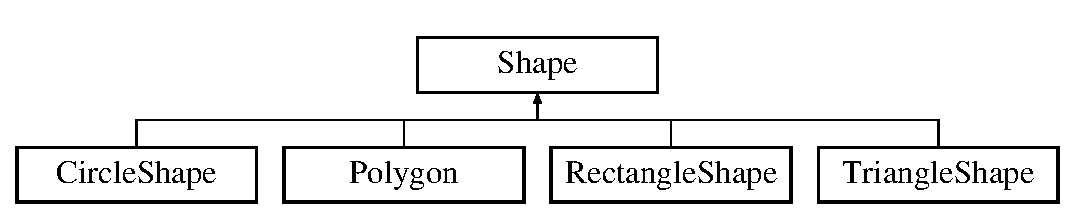
\includegraphics[height=2.000000cm]{class_shape}
\end{center}
\end{figure}
\subsection*{Public Member Functions}
\begin{DoxyCompactItemize}
\item 
\hypertarget{class_shape_a402c108e2d1a078a1974b3ecc7a32fc6}{}\label{class_shape_a402c108e2d1a078a1974b3ecc7a32fc6} 
void {\bfseries set\+Position} (\hyperlink{struct_p_vector}{P\+Vector})
\item 
\hypertarget{class_shape_adeca39958a7adbb8c80f5af9cf5f60bd}{}\label{class_shape_adeca39958a7adbb8c80f5af9cf5f60bd} 
void {\bfseries set\+Position} (float, float)
\item 
\hypertarget{class_shape_aeabb7a6bd05635c30fa56e31766b09bc}{}\label{class_shape_aeabb7a6bd05635c30fa56e31766b09bc} 
void {\bfseries set\+Color} (\hyperlink{struct_color}{Color})
\item 
\hypertarget{class_shape_a11a5311064e9504e1acfdd91ec94882d}{}\label{class_shape_a11a5311064e9504e1acfdd91ec94882d} 
void {\bfseries set\+Color} (float, float, float, float)
\item 
\hypertarget{class_shape_a12f4452300d4321762fbf466e37190e0}{}\label{class_shape_a12f4452300d4321762fbf466e37190e0} 
\hyperlink{struct_p_vector}{P\+Vector} {\bfseries get\+Position} ()
\item 
\hypertarget{class_shape_ab20c5a85d59e7b9d0164158f4ad6c2a4}{}\label{class_shape_ab20c5a85d59e7b9d0164158f4ad6c2a4} 
\hyperlink{struct_color}{Color} {\bfseries get\+Color} ()
\end{DoxyCompactItemize}
\subsection*{Protected Attributes}
\begin{DoxyCompactItemize}
\item 
\hypertarget{class_shape_afb4e17803a82f3144777cd249480cb91}{}\label{class_shape_afb4e17803a82f3144777cd249480cb91} 
\hyperlink{struct_p_vector}{P\+Vector} {\bfseries position}
\item 
\hypertarget{class_shape_ac56e2bf5eb24cf37b6e08c671501566b}{}\label{class_shape_ac56e2bf5eb24cf37b6e08c671501566b} 
\hyperlink{struct_color}{Color} {\bfseries color}
\end{DoxyCompactItemize}


The documentation for this class was generated from the following files\+:\begin{DoxyCompactItemize}
\item 
Tools.\+hpp\item 
Tools.\+cpp\end{DoxyCompactItemize}

\hypertarget{class_triangle_shape}{}\section{Triangle\+Shape Class Reference}
\label{class_triangle_shape}\index{Triangle\+Shape@{Triangle\+Shape}}
Inheritance diagram for Triangle\+Shape\+:\begin{figure}[H]
\begin{center}
\leavevmode
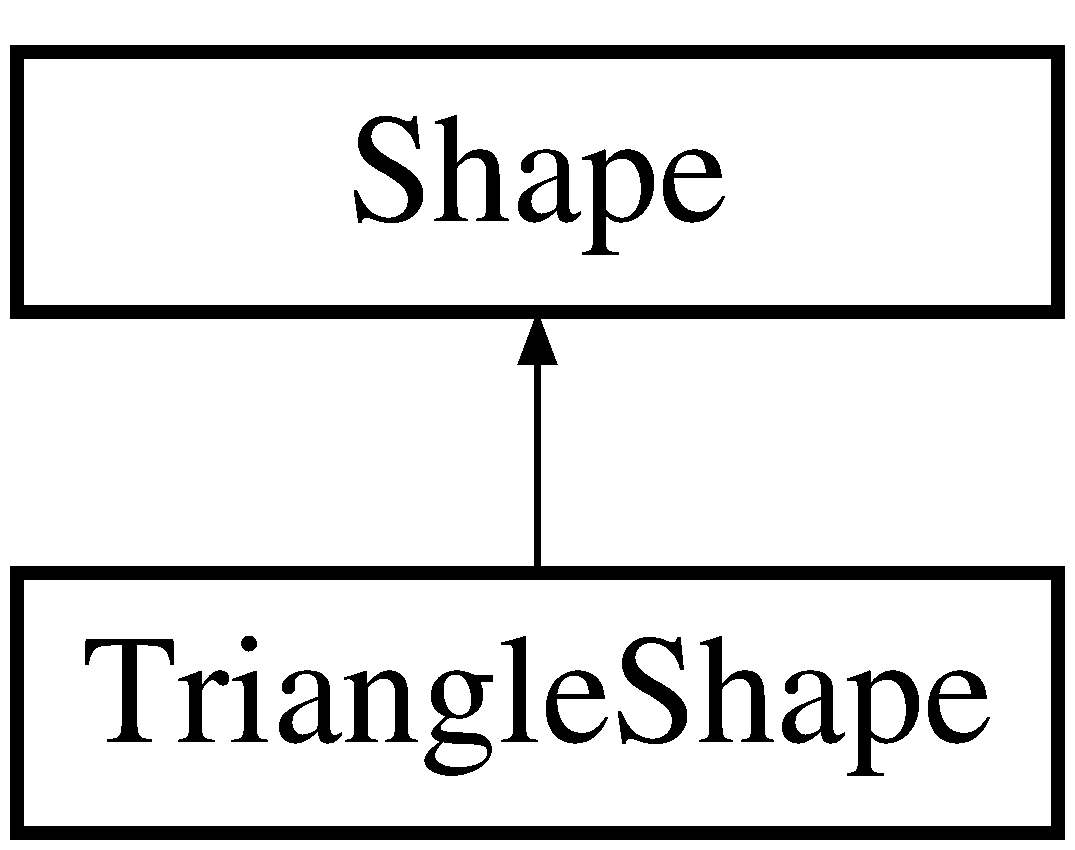
\includegraphics[height=2.000000cm]{class_triangle_shape}
\end{center}
\end{figure}
\subsection*{Public Member Functions}
\begin{DoxyCompactItemize}
\item 
\hypertarget{class_triangle_shape_a0742fc5cefcf87ec714df887eac1063b}{}\label{class_triangle_shape_a0742fc5cefcf87ec714df887eac1063b} 
{\bfseries Triangle\+Shape} (float, float, float, float)
\item 
\hypertarget{class_triangle_shape_a1405e2b1b5d9c9e8283156eec6cbf021}{}\label{class_triangle_shape_a1405e2b1b5d9c9e8283156eec6cbf021} 
void {\bfseries draw\+Fill} ()
\item 
\hypertarget{class_triangle_shape_add481f7167360aeeaf411d714c9d68be}{}\label{class_triangle_shape_add481f7167360aeeaf411d714c9d68be} 
void {\bfseries draw\+Outline} ()
\item 
\hypertarget{class_triangle_shape_abd78b976444ddf526b839a5d4706ff5c}{}\label{class_triangle_shape_abd78b976444ddf526b839a5d4706ff5c} 
void {\bfseries set\+Size} (\hyperlink{struct_p_vector}{P\+Vector})
\item 
\hypertarget{class_triangle_shape_aa0d2b84703d859f14c73023315bd3896}{}\label{class_triangle_shape_aa0d2b84703d859f14c73023315bd3896} 
\hyperlink{struct_p_vector}{P\+Vector} {\bfseries get\+Size} ()
\end{DoxyCompactItemize}
\subsection*{Additional Inherited Members}


The documentation for this class was generated from the following files\+:\begin{DoxyCompactItemize}
\item 
Tools.\+hpp\item 
Tools.\+cpp\end{DoxyCompactItemize}

\chapter{File Documentation}
\hypertarget{_tools_8cpp}{}\section{Tools.\+cpp File Reference}
\label{_tools_8cpp}\index{Tools.\+cpp@{Tools.\+cpp}}
{\ttfamily \#include \char`\"{}Tools.\+hpp\char`\"{}}\newline
\subsection*{Functions}
\begin{DoxyCompactItemize}
\item 
\hyperlink{struct_p_vector}{P\+Vector} \hyperlink{_tools_8cpp_a6e17894a9656f2b9fd133435002d4090}{operator+} (\hyperlink{struct_p_vector}{P\+Vector} a, \hyperlink{struct_p_vector}{P\+Vector} b)
\item 
\hyperlink{struct_p_vector}{P\+Vector} \hyperlink{_tools_8cpp_a711e54ed79aa57771cf76101cfd2acd4}{operator-\/} (\hyperlink{struct_p_vector}{P\+Vector} a, \hyperlink{struct_p_vector}{P\+Vector} b)
\item 
\hyperlink{struct_p_vector}{P\+Vector} \hyperlink{_tools_8cpp_a159c7545056fcb94fac1a0bb168c2420}{operator$\ast$} (\hyperlink{struct_p_vector}{P\+Vector} a, \hyperlink{struct_p_vector}{P\+Vector} b)
\item 
\hyperlink{struct_p_vector}{P\+Vector} \hyperlink{_tools_8cpp_a17103104488fea43b4d560c39ea6350a}{operator/} (\hyperlink{struct_p_vector}{P\+Vector} a, \hyperlink{struct_p_vector}{P\+Vector} b)
\item 
\hyperlink{struct_p_vector}{P\+Vector} \hyperlink{_tools_8cpp_a8ca522b6a7133fdb2a9e213e3ee8547c}{get\+Mouse\+Position} ()
\end{DoxyCompactItemize}


\subsection{Function Documentation}
\hypertarget{_tools_8cpp_a8ca522b6a7133fdb2a9e213e3ee8547c}{}\label{_tools_8cpp_a8ca522b6a7133fdb2a9e213e3ee8547c} 
\index{Tools.\+cpp@{Tools.\+cpp}!get\+Mouse\+Position@{get\+Mouse\+Position}}
\index{get\+Mouse\+Position@{get\+Mouse\+Position}!Tools.\+cpp@{Tools.\+cpp}}
\subsubsection{\texorpdfstring{get\+Mouse\+Position()}{getMousePosition()}}
{\footnotesize\ttfamily \hyperlink{struct_p_vector}{P\+Vector} get\+Mouse\+Position (\begin{DoxyParamCaption}{ }\end{DoxyParamCaption})}

\hypertarget{_tools_8cpp_a159c7545056fcb94fac1a0bb168c2420}{}\label{_tools_8cpp_a159c7545056fcb94fac1a0bb168c2420} 
\index{Tools.\+cpp@{Tools.\+cpp}!operator$\ast$@{operator$\ast$}}
\index{operator$\ast$@{operator$\ast$}!Tools.\+cpp@{Tools.\+cpp}}
\subsubsection{\texorpdfstring{operator$\ast$()}{operator*()}}
{\footnotesize\ttfamily \hyperlink{struct_p_vector}{P\+Vector} operator$\ast$ (\begin{DoxyParamCaption}\item[{\hyperlink{struct_p_vector}{P\+Vector}}]{a,  }\item[{\hyperlink{struct_p_vector}{P\+Vector}}]{b }\end{DoxyParamCaption})}

\hypertarget{_tools_8cpp_a6e17894a9656f2b9fd133435002d4090}{}\label{_tools_8cpp_a6e17894a9656f2b9fd133435002d4090} 
\index{Tools.\+cpp@{Tools.\+cpp}!operator+@{operator+}}
\index{operator+@{operator+}!Tools.\+cpp@{Tools.\+cpp}}
\subsubsection{\texorpdfstring{operator+()}{operator+()}}
{\footnotesize\ttfamily \hyperlink{struct_p_vector}{P\+Vector} operator+ (\begin{DoxyParamCaption}\item[{\hyperlink{struct_p_vector}{P\+Vector}}]{a,  }\item[{\hyperlink{struct_p_vector}{P\+Vector}}]{b }\end{DoxyParamCaption})}

\hypertarget{_tools_8cpp_a711e54ed79aa57771cf76101cfd2acd4}{}\label{_tools_8cpp_a711e54ed79aa57771cf76101cfd2acd4} 
\index{Tools.\+cpp@{Tools.\+cpp}!operator-\/@{operator-\/}}
\index{operator-\/@{operator-\/}!Tools.\+cpp@{Tools.\+cpp}}
\subsubsection{\texorpdfstring{operator-\/()}{operator-()}}
{\footnotesize\ttfamily \hyperlink{struct_p_vector}{P\+Vector} operator-\/ (\begin{DoxyParamCaption}\item[{\hyperlink{struct_p_vector}{P\+Vector}}]{a,  }\item[{\hyperlink{struct_p_vector}{P\+Vector}}]{b }\end{DoxyParamCaption})}

\hypertarget{_tools_8cpp_a17103104488fea43b4d560c39ea6350a}{}\label{_tools_8cpp_a17103104488fea43b4d560c39ea6350a} 
\index{Tools.\+cpp@{Tools.\+cpp}!operator/@{operator/}}
\index{operator/@{operator/}!Tools.\+cpp@{Tools.\+cpp}}
\subsubsection{\texorpdfstring{operator/()}{operator/()}}
{\footnotesize\ttfamily \hyperlink{struct_p_vector}{P\+Vector} operator/ (\begin{DoxyParamCaption}\item[{\hyperlink{struct_p_vector}{P\+Vector}}]{a,  }\item[{\hyperlink{struct_p_vector}{P\+Vector}}]{b }\end{DoxyParamCaption})}


\hypertarget{_tools_8hpp}{}\section{Tools.\+hpp File Reference}
\label{_tools_8hpp}\index{Tools.\+hpp@{Tools.\+hpp}}
{\ttfamily \#include $<$vector$>$}\newline
{\ttfamily \#include \char`\"{}sl.\+h\char`\"{}}\newline
\subsection*{Classes}
\begin{DoxyCompactItemize}
\item 
struct \hyperlink{struct_p_vector}{P\+Vector}
\item 
struct \hyperlink{struct_color}{Color}
\item 
class \hyperlink{class_shape}{Shape}
\item 
class \hyperlink{class_circle_shape}{Circle\+Shape}
\item 
class \hyperlink{class_rectangle_shape}{Rectangle\+Shape}
\item 
class \hyperlink{class_triangle_shape}{Triangle\+Shape}
\item 
class \hyperlink{class_polygon}{Polygon}
\end{DoxyCompactItemize}
\subsection*{Functions}
\begin{DoxyCompactItemize}
\item 
\hyperlink{struct_p_vector}{P\+Vector} \hyperlink{_tools_8hpp_aafadb01ae495c1349d302aab44627074}{operator+} (\hyperlink{struct_p_vector}{P\+Vector}, \hyperlink{struct_p_vector}{P\+Vector})
\item 
\hyperlink{struct_p_vector}{P\+Vector} \hyperlink{_tools_8hpp_a6a87b585d9013e04bc2427208aa2395f}{operator-\/} (\hyperlink{struct_p_vector}{P\+Vector}, \hyperlink{struct_p_vector}{P\+Vector})
\item 
\hyperlink{struct_p_vector}{P\+Vector} \hyperlink{_tools_8hpp_a2049861687599317eaa56f60f33e9ef5}{operator$\ast$} (\hyperlink{struct_p_vector}{P\+Vector}, \hyperlink{struct_p_vector}{P\+Vector})
\item 
\hyperlink{struct_p_vector}{P\+Vector} \hyperlink{_tools_8hpp_ac1d3ae324f231b1dc842158a08230f5a}{operator/} (\hyperlink{struct_p_vector}{P\+Vector}, \hyperlink{struct_p_vector}{P\+Vector})
\item 
\hyperlink{struct_p_vector}{P\+Vector} \hyperlink{_tools_8hpp_a8ca522b6a7133fdb2a9e213e3ee8547c}{get\+Mouse\+Position} ()
\end{DoxyCompactItemize}


\subsection{Function Documentation}
\hypertarget{_tools_8hpp_a8ca522b6a7133fdb2a9e213e3ee8547c}{}\label{_tools_8hpp_a8ca522b6a7133fdb2a9e213e3ee8547c} 
\index{Tools.\+hpp@{Tools.\+hpp}!get\+Mouse\+Position@{get\+Mouse\+Position}}
\index{get\+Mouse\+Position@{get\+Mouse\+Position}!Tools.\+hpp@{Tools.\+hpp}}
\subsubsection{\texorpdfstring{get\+Mouse\+Position()}{getMousePosition()}}
{\footnotesize\ttfamily \hyperlink{struct_p_vector}{P\+Vector} get\+Mouse\+Position (\begin{DoxyParamCaption}{ }\end{DoxyParamCaption})}

\hypertarget{_tools_8hpp_a2049861687599317eaa56f60f33e9ef5}{}\label{_tools_8hpp_a2049861687599317eaa56f60f33e9ef5} 
\index{Tools.\+hpp@{Tools.\+hpp}!operator$\ast$@{operator$\ast$}}
\index{operator$\ast$@{operator$\ast$}!Tools.\+hpp@{Tools.\+hpp}}
\subsubsection{\texorpdfstring{operator$\ast$()}{operator*()}}
{\footnotesize\ttfamily \hyperlink{struct_p_vector}{P\+Vector} operator$\ast$ (\begin{DoxyParamCaption}\item[{\hyperlink{struct_p_vector}{P\+Vector}}]{,  }\item[{\hyperlink{struct_p_vector}{P\+Vector}}]{ }\end{DoxyParamCaption})}

\hypertarget{_tools_8hpp_aafadb01ae495c1349d302aab44627074}{}\label{_tools_8hpp_aafadb01ae495c1349d302aab44627074} 
\index{Tools.\+hpp@{Tools.\+hpp}!operator+@{operator+}}
\index{operator+@{operator+}!Tools.\+hpp@{Tools.\+hpp}}
\subsubsection{\texorpdfstring{operator+()}{operator+()}}
{\footnotesize\ttfamily \hyperlink{struct_p_vector}{P\+Vector} operator+ (\begin{DoxyParamCaption}\item[{\hyperlink{struct_p_vector}{P\+Vector}}]{,  }\item[{\hyperlink{struct_p_vector}{P\+Vector}}]{ }\end{DoxyParamCaption})}

\hypertarget{_tools_8hpp_a6a87b585d9013e04bc2427208aa2395f}{}\label{_tools_8hpp_a6a87b585d9013e04bc2427208aa2395f} 
\index{Tools.\+hpp@{Tools.\+hpp}!operator-\/@{operator-\/}}
\index{operator-\/@{operator-\/}!Tools.\+hpp@{Tools.\+hpp}}
\subsubsection{\texorpdfstring{operator-\/()}{operator-()}}
{\footnotesize\ttfamily \hyperlink{struct_p_vector}{P\+Vector} operator-\/ (\begin{DoxyParamCaption}\item[{\hyperlink{struct_p_vector}{P\+Vector}}]{,  }\item[{\hyperlink{struct_p_vector}{P\+Vector}}]{ }\end{DoxyParamCaption})}

\hypertarget{_tools_8hpp_ac1d3ae324f231b1dc842158a08230f5a}{}\label{_tools_8hpp_ac1d3ae324f231b1dc842158a08230f5a} 
\index{Tools.\+hpp@{Tools.\+hpp}!operator/@{operator/}}
\index{operator/@{operator/}!Tools.\+hpp@{Tools.\+hpp}}
\subsubsection{\texorpdfstring{operator/()}{operator/()}}
{\footnotesize\ttfamily \hyperlink{struct_p_vector}{P\+Vector} operator/ (\begin{DoxyParamCaption}\item[{\hyperlink{struct_p_vector}{P\+Vector}}]{,  }\item[{\hyperlink{struct_p_vector}{P\+Vector}}]{ }\end{DoxyParamCaption})}


%--- End generated contents ---

% Index
\backmatter
\newpage
\phantomsection
\clearemptydoublepage
\addcontentsline{toc}{chapter}{Index}
\printindex

\end{document}
